\section{Kabinet}

For at øge SPL for højtalerens resonansfrekvens, sættes højtaleren i et lukket kabinet der er designet til formålet.
Kabinettets ønskede volumen kan findes i databladet for højtaleren\cite{FW168} som ækvivalent volumen $V_{as} = 16.5L$. Ved denne højtalervolumen vil resonansfrekvensen $f_s$ dog øges med ca. $41\%$ da den indskudte masse af luften vil give højtaleren mindre bevægelsesfrihed. Dvs $f_{kabinet}=45Hz\cdot1.45=63.45Hz$. 

Den akustiske model for et lukket kabinet er lig figur \ref{fig:BR_a_Model} uden $M_{AP}$. Det lukkede kabinets resonansfrekvens kan derfor udregnes med ligning \ref{lig:fckabinet}.

Med et basreflekskabinet vil man udover kabinetets resonansfrekvens $(f_{kabinet})$ tilføje endnu en resonansfrekvens for porten $(f_{port})$,da man med luftmassen i porten, vil skabe en fjedervirkning som sammen med kabinettets indespærrede luft kan afstemmes til en given resonansfrekvens. For størst effekt, bør denne resonans afstemmes til højtalerens resonansfrekvens $f_s = 45Hz$.

Realiseringen af basreflekskabinettet har medført et kabinet, hvis indre totalvolumen er $V_{total}=17.8L$. Dette skyldes at der inde i kabinettet er tre genstande som optager rumfang som derfor ikke skal medregnes i den totale luftvolumen. Det er højtaleren, porten samt en stabiliseringspind. Disse tre genstande har et volumen på ialt $V_{fyld}=1.3L$. Det totale luftvolumen rammer dermed $V_{total}-V_{fyld}=16.5L=V_{as}$.

Portens resonansfrekvens findes med ligning \ref{lig:fport}
\begin{equation}\label{lig:fport}
f_{port}=\frac{1}{2 \pi \sqrt{M_{AP} C_{AB}}}
\end{equation}
Hvor $M_{AP}$ er portens akustiske luftmasse og $C_{AB}$ er massen af kabinettets akustiske luftvolumen.
\begin{equation}\label{lig:CAB}
C_{AB}=\frac{V_{as}}{\rho c^2}
	\end{equation}
	Hvor luftens massefylde er $\rho=1.18 \frac{kg}{m^3}$ 
\begin{equation}\label{lig:MAP}
M_{AP}=\frac{\rho}{S_P} (L_P+1.5\sqrt{\frac{S_P}{\pi}})
\end{equation}	
Hvor portens areal her er bestemt til $S_P=2cm^2$

Indsætter man ligning \ref{lig:MAP} i ligning \ref{lig:fport} og løser for $f_{port}=45Hz$ får man portens længde til 13.91cm (Realiseret med 14cm)


Resonansfrekvensen for kabinettet udregnes i ligning \ref{lig:fckabinet}, hvilket er tæt på de $41\%$ ekstra.
\begin{equation}\label{lig:fckabinet}
f_{kabinet}=\frac{1}{2 \pi \sqrt{M_{AS} \cdot C_{AS}||C_{AB}}} = 64.57Hz
\end{equation}
\begin{figure}[H]
	\centering
	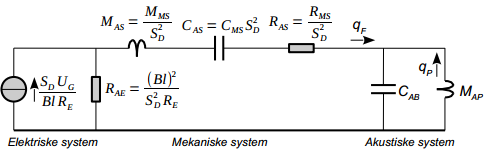
\includegraphics[width=\textwidth]{Pics/Akustisk_basrefleks_model.PNG}
	\label{fig:BR_a_Model}
	\caption{Akustisk model for højtaler i basreflekskabinet \cite{Elektroakustik}} 
\end{figure}

Til realiseringen bruges også basrefleksporte på hhv. 7cm og 3.5cms længde. Når disse bruges til målinger, vil de både ændre på portens resonans (pga ændret portvolumen), samt på kabinettets resonansfrekvens (pga mindre rumfang af selve porten.)

I tabel \ref{tab:resonansfreq} ses de udregnede resonansfrekvenser for både kabinet og port ved forskellige portlængder.

\begin{table}[h]
	\centering
	\begin{tabular}{|c|c|c|}
		\hline	
		\textbf{Længde af port} & \textbf{$f_{kabinet}$} & \textbf{$f_{port}$} \\\hline
		$14cm$ & $64.5Hz$ & $44.8Hz$ \\\hline
		$7cm$ & $64.4Hz$ & $57.3Hz$ \\\hline
		$3.5cm$ & $64.3Hz$ & $69.6Hz$ \\\hline
		$0cm$ & $64.2Hz$ & - \\\hline
		
	\end{tabular}
	\label{tab:resonansfreq}
	\caption{Teoretiske resonansfrekvenser for den realiserede basreflekskabinet v. forskellige portlængder.}
\end{table} 